\documentclass[a4paper, 12pt]{article}

%%% Работа с русским языком
\usepackage{cmap}					% поиск в PDF
\usepackage{mathtext} 				% русские буквы в формулах
\usepackage[T2A]{fontenc}			% кодировка
\usepackage[utf8]{inputenc}			% кодировка исходного текста
\usepackage[russian]{babel}	% локализация и переносы

%%% Дополнительная работа с математикой
\usepackage{amsmath,amsfonts,amssymb,amsthm,mathtools} % AMS
\usepackage{icomma} % "Умная" запятая: $0,2$ --- число, $0, 2$ --- перечисление

%% Номера формул
%\mathtoolsset{showonlyrefs=true} % Показывать номера только у тех формул, на которые есть \eqref{} в тексте.

%% Шрифты
\usepackage{euscript}	 % Шрифт Евклид
\usepackage{mathrsfs} % Красивый матшрифт

%% Поля
\usepackage[left=2cm,right=2cm,top=2cm,bottom=2cm,bindingoffset=0cm]{geometry}

%% Русские списки
\usepackage{enumitem}
\makeatletter
\AddEnumerateCounter{\asbuk}{\russian@alph}{щ}
\makeatother

%%% Работа с картинками
\usepackage{graphicx}  % Для вставки рисунков
\graphicspath{{images/}{images2/}}  % папки с картинками
\setlength\fboxsep{3pt} % Отступ рамки \fbox{} от рисунка
\setlength\fboxrule{1pt} % Толщина линий рамки \fbox{}
\usepackage{wrapfig} % Обтекание рисунков и таблиц текстом

%%% Работа с таблицами
\usepackage{array,tabularx,tabulary,booktabs} % Дополнительная работа с таблицами
\usepackage{longtable}  % Длинные таблицы
\usepackage{multirow} % Слияние строк в таблице

%% Красная строка
\setlength{\parindent}{2em}

%% Интервалы
\linespread{1}
\usepackage{multirow}

%% TikZ
\usepackage{tikz}
\usetikzlibrary{graphs,graphs.standard}

%% Верхний колонтитул
\usepackage{fancyhdr}
\pagestyle{fancy}

%% Перенос знаков в формулах (по Львовскому)
\newcommand*{\hm}[1]{#1\nobreak\discretionary{}
	{\hbox{$\mathsurround=0pt #1$}}{}}

%% Мои дополнения
\usepackage{float} %Добавляет возможность работы с командой [H] которая улучшает расположение на странице
\usepackage{gensymb} %Красивые градусы
\usepackage{graphicx}               % Импорт изображений
\usepackage{caption} % Пакет для подписей к рисункам, в частности, для работы caption*

% подключаем hyperref (для ссылок внутри  pdf)
\usepackage[unicode, pdftex]{hyperref}

%%% Теоремы
\theoremstyle{plain}                    % Это стиль по умолчанию, его можно не переопределять.
\renewcommand\qedsymbol{$\blacksquare$} % переопределение символа завершения доказательства

\newtheorem{theorem}{Теорема}[section] % Теорема (счетчик по секиям)
\newtheorem{proposition}{Утверждение}[section] % Утверждение (счетчик по секиям)
\newtheorem{definition}{Определение}[section] % Определение (счетчик по секиям)
\newtheorem{corollary}{Следствие}[theorem] % Следстиве (счетчик по теоремам)
\newtheorem{problem}{Задача}[section] % Задача (счетчик по секиям)
\newtheorem*{remark}{Примечание} % Примечание (можно переопределить, как Замечание)
\newtheorem{lemma}{Лемма}[section] % Лемма (счетчик по секиям)
% % \newcommand{\eqdef}{\stackrel{\mathrm{def}}{=}}
% \newcommand{\ryad}{\sum\limits^{\infty}_{k = 0}}

% \newcommand{\R}{\mathbb{R}}
% \newcommand{\N}{\mathbb{N}}
% \newcommand{\series}{\sum\limits_{k=1}^{\infty}}
% \newcommand{\useries}{\sum\limits_{k=1}^{\infty} u_k}
% \newcommand{\useriesl}{\sum\limits_{k=1}^{\infty} u_k < \infty}
% \newcommand{\useriese}{\sum\limits_{k=1}^{\infty} u_k = \infty}
% \newcommand{\auseries}{\sum\limits_{k=1}^{\infty} |u_k|}
% \newcommand{\auseriesl}{\sum\limits_{k=1}^{\infty} |u_k| < \infty}
% \newcommand{\auseriese}{\sum\limits_{k=1}^{\infty} |u_k| = \infty}
% \newcommand{\sn}{\sum\limits_{k=1}^{n} u_k}

% \renewcommand {\ge}{\geqslant}
% \renewcommand {\le}{\leqslant}
% \renewcommand {\geq}{\geqslant}
% \renewcommand {\leq}{\leqslant}
% \renewcommand {\epsilon}{\varepsilon}

\begin{document}
    \newcommand{\HRule}{\rule{\linewidth}{0.7mm}} % Defines a new command for the horizontal lines, change thickness here
	
	\begin{center}
		\large\textbf{Московский Физико-Технический Институт}\\ % Name of your university/college
		\large\textbf{(государственный университет)}
	
		\vfill
		
		\Large Лабораторная работа по курсу общей физики № *labnum*\\[0.5cm] % Preambule of your document title
		
		
		\HRule
		\\[0.4cm]
		{ \huge \bfseries *name of your labwork*}% Title of your document
		\\[0.4cm] 
		\HRule
		\\[0.5cm]
		
		\ \\
	\textbf{\large Автор:} \\	
	\large *your name* *groupname*\\ % Your name and something more, your group num for example
		\vfill
		\hspace*{-0.8 cm}
\includegraphics[width=100 pt]{frkt_logo}\\ % logo of your  company/university/college
		\large Долгопрудный, 2021 % location and year
	\end{center}

\newpage
\setcounter{page}{2}
\fancyfoot[c]{\thepage}
\fancyhead[L] {Работа № *labnum*} % some information in page header
\fancyhead[R]{}

    Запишем закон Кюри-Вейесса

    \begin{equation}
        \chi \propto \frac{1}{T - \theta_p}
    \end{equation}

    \noindent где $\theta_p$ -- параметр размерности температуры. Закон Кюри-Вейесса хорошо выполняется вдали от $\theta_K$ -- 
    температуры Кюри, однако нарушается при $T \rightarrow \theta_K$. Поэтому параметр $\theta_p$ отличается от температуры Кюри
    (как правило $\theta_K < theta_p$). На практике наблюдается картина, изображенная на \hyperref[theory_xi]{рисунке}.

    \begin{figure}
        \centering
        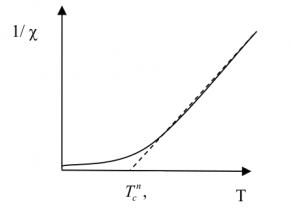
\includegraphics[scale = 0.75]{theory.png}
        \caption{Зависимость обратной магнитной восприимчивости от температуры}
        \label{theory_xi}
    \end{figure}

    Для практического исследования будем применять формулу

    \begin{equation}
        \frac{1}{\chi} \propto (T - \theta_p) \propto \frac{1}{\tau^2 - \tau_0^2}
    \end{equation}

    \noindent $\tau$ -- период колебания автогениратора, $\tau_0$ -- период колебаний автогениратора в отсутствии исследуемого
    образца.

    Запишем параметры установки

    \begin{center}
        $\tau_0 = 9,045$ мкс -- период колебаний автогениратора в отсутствии исследуемого образца \\
        $L_0 = 1602$ мкГн -- индуктивность в отсутствии исследуемого образца \\
        $k = 24$ град/мВ -- чувствительность термопары \\
    \end{center}

    Отсюда посчитаем точность определения температуры

    \[ 24 \cdot 3 \cdot 10^{-3} ~ \text{мВ} = 0,072 ~ C^{o} \]

    Выражение для индуктивности тороидальной катушки в СИ

    \begin{equation}
        L = \frac{\mu_0 \mu N}{2 \pi R} S
    \end{equation}

    Период колебаний по формуле Джоуля-Томсона

    \begin{equation}
        \tau = 2 \pi \sqrt{L C}
    \end{equation}

    \begin{equation}
        \frac{\tau^2 - \tau_0^2}{\tau_0^2} = \frac{\tau^2}{\tau_0^2} - 1 = \frac{\mu}{\mu_0} - 1 = \mu - 1 = \chi        
    \end{equation}

    Таким образом, получаем

    \begin{equation}
        \chi = \frac{\tau^2}{\tau_0^2} - 1
    \end{equation}

    \begin{table}[]
    \begin{center}
        \begin{tabular}{|c|c|c|c|c|c|c|}
            \hline
            $t, ~ C^o$ & $\tau$, мкс & $\chi$    & $1/\chi$  & $T, ~ K$ & $\mu$    & $L$, мкГн  \\ \hline
            10,77      & 10,86101    & 0,44186   & 2,26315   & 283,92   & 1,44186  & 2309,86073  \\ \hline
            12,12      & 10,8358     & 0,43517   & 2,29792   & 285,27   & 1,43517  & 2299,15012  \\ \hline
            14,14      & 10,76926    & 0,41760   & 2,39461   & 287,29   & 1,41760  & 2270,99978  \\ \hline
            16,13      & 10,66155    & 0,38938   & 2,56813   & 289,28   & 1,38938  & 2225,79962  \\ \hline
            18,12      & 10,4786     & 0,34211   & 2,92300   & 291,27   & 1,34211  & 2150,06650  \\ \hline
            20,11      & 10,17474    & 0,26540   & 3,76782   & 293,26   & 1,26540  & 2027,17858  \\ \hline
            22,1       & 9,79891     & 0,17364   & 5,75872   & 295,25   & 1,17364  & 1880,18640  \\ \hline
            24,1       & 9,52033     & 0,10786   & 9,27084   & 297,25   & 1,10786  & 1774,79981  \\ \hline
            26,1       & 9,39631     & 0,07918   & 12,6280   & 299,25   & 1,07918  & 1728,86086  \\ \hline
            30,09      & 9,27918     & 0,05245   & 19,0652   & 303,24   & 1,05245  & 1686,02716  \\ \hline
        \end{tabular}
    \end{center}
    \caption{Экспериментальные данные}
    \label{experiment_table}
\end{table}

    Используя данные, полученные при проведении эксперимента, построим графики зависимости \hyperref[graph_1x(T)]{$1/\chi(T)$},
    \hyperref[graph_x_mu_(T)]{$\chi(T)$}, \hyperref[graph_x_mu_(T)]{$\mu(T)$} и \hyperref[graph_L(T)]{$L(T)$}.

    \begin{figure}
        \centering
        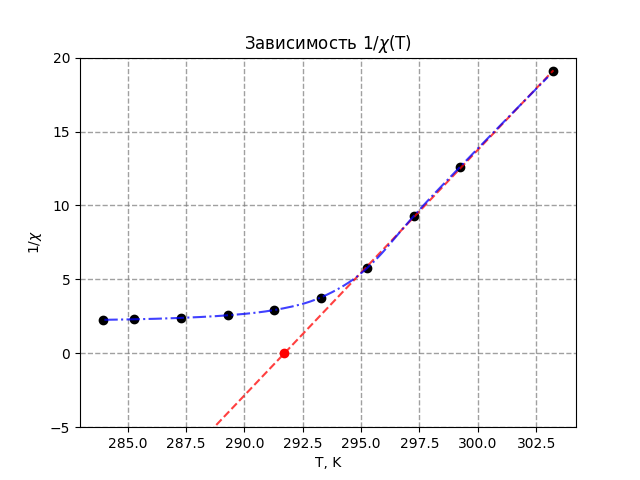
\includegraphics[width = \linewidth]{graph_1x(T).png}
        \caption{Зависимость обратной магнитной восприимчивости от температуры}
        \label{graph_1x(T)}
    \end{figure}

    \begin{figure}
        \centering
        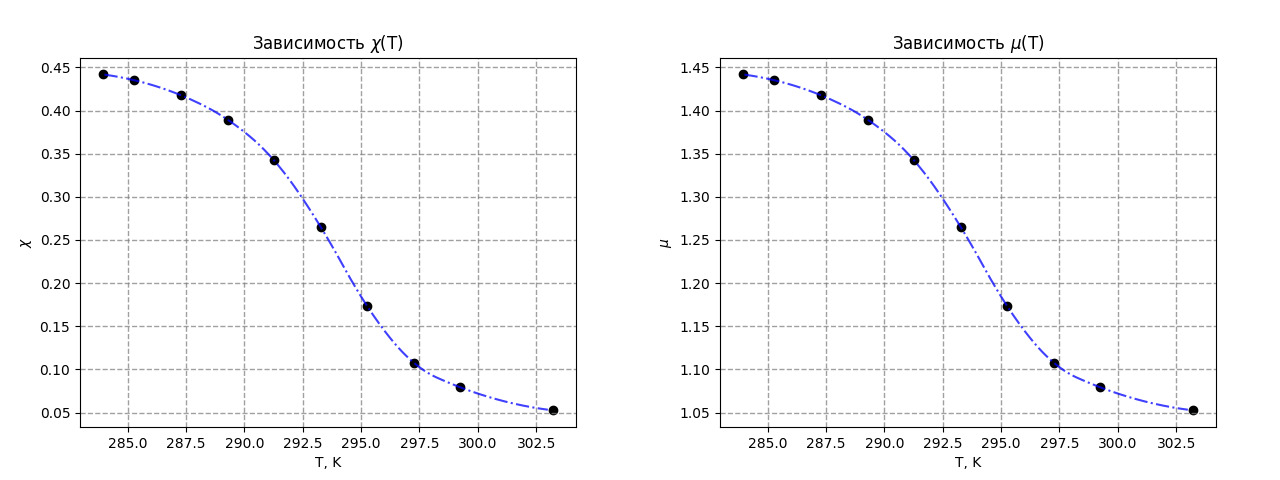
\includegraphics[width=\linewidth]{imgonline-com-ua-2to1-spGCn2gxrV.jpg}
        \caption{Графики зависимости магнитной восприимчивости и магнитной проницаемости от температуры}
        \label{graph_x_mu_(T)}
    \end{figure}

    \begin{figure}[h!]
        \centering
        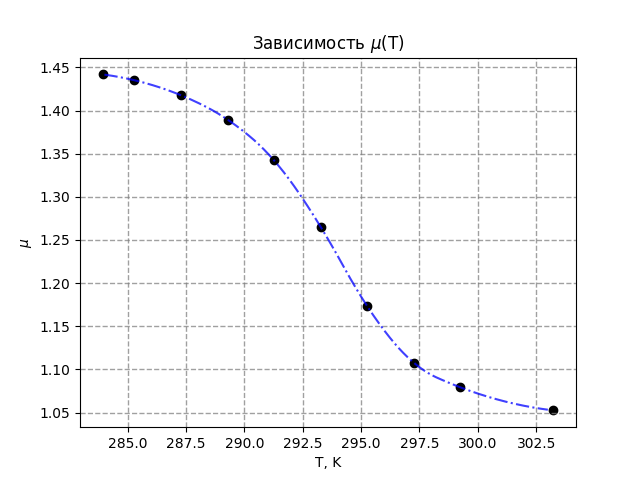
\includegraphics[width=\linewidth]{graph_L(T).png}
        \label{graph_L(T)}
        \caption{Зависимость индуктивности от температуры}
    \end{figure}

    Используя эксперементальные данные и графики получаем значение параметра $\theta_p$:

    \begin{center}
        \fbox{$\theta_p = 291 ~ K = 18 ~ C^o$}
    \end{center}

\end{document}